\section{Kontrollstrukturen \verweis{8}}
	\begin{minipage}[t]{9 cm}
		\subsection{Sequenz \verweis{8.1}}
			Die Sequenz ist eine zeitlich geordnete Abfolge von Anweisungen. \\
				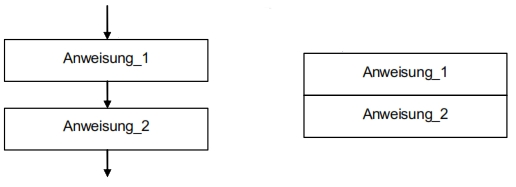
\includegraphics[width=1\textwidth]{pics/Sequenz.jpg}	
			
	\end{minipage}
	%
	\begin{minipage}[t]{9 cm}
			\subsubsection{Block}
				\begin{compactitem}
					\item Erfordert die Syntax genau eine Anweisung, so können dennoch mehrere Anweisungen geschrieben werden, wenn man sie in Form eines Blocks zusammenfasst.
					\item Ein Block wird mit geschweiften Klammern eingefasst. $\{ \dots \}$ Ein Block zählt syntaktisch als eine einzige Anweisung.
				\end{compactitem}
				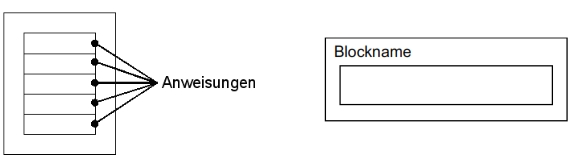
\includegraphics[width=1\textwidth]{pics/Block.jpg}
	\end{minipage}	
		
	\subsection{Selektion \verweis{8.2}}
		Von \textbf{Selektion} spricht man zum einen, wenn man eine Anweisung nur dann ausführen will, wenn eine bestimmte Bedingung zutrifft. Zum anderen möchte man mit Selektionsanweisungen zwischen zwei Möglichkeiten (entweder/oder) bzw. zwischen mehreren Möglichkeiten genau eine auswählen.
		
		\begin{minipage}[t]{5.5 cm}
			\subsubsection{Einfache Alternative}
				\lstinputlisting[language=C,tabsize=2]{code/strukturen_if_else.c}
		\end{minipage}
		%
		\begin{minipage}[t]{5.5 cm}
			\subsubsection{Bedingte Anweisung}
				\lstinputlisting[language=C,tabsize=2]{code/strukturen_if.c}
		\end{minipage}
		%
		\begin{minipage}[t]{7 cm}
			\subsubsection{Mehrfache Alternative - else if}
				\lstinputlisting[language=C,tabsize=2]{code/strukturen_else_if.c}
		\end{minipage}